\section{Experimental Evaluation}
\label{chap3-sec:experiments}
Based on the performance guarantees summarized in Tables~\ref{chap3-tab:upper_bounds_triangle} and \ref{chap3-tab:upper_bounds_4cycle}, we pose the following research questions: 

\begin{description}[leftmargin=8.75mm]
% \begin{description}[leftmargin=9.75mm]
% \begin{itemize}[leftmargin=9.7mm]
    \item[RQ1.] 
    %\item 
    How much do our entire algorithms (\AlgWSTriVR{} and \AlgWSCyc{}) outperform the local algorithms?
    %How much do our shuffle algorithms (\AlgWSTriVR{} and \AlgWSCyc{}) reduce the estimation error, compared to the local algorithms?
    \item[RQ2.] 
    %\item 
    For triangles, how much does our variance reduction technique decrease the relative error?
    \item[RQ3.] 
    %\item 
    How small relative errors do our entire algorithms 
    % (\AlgWSTriVR{} and \AlgWSCyc{}) 
    achieve with a small privacy budget?
\end{description}
% \end{itemize}
We designed experiments to answer these questions. 

\subsection{Experimental Set-up}
\label{chap3-sub:set-up}
We used the following two real graph datasets: 
\begin{itemize}
    \item \textbf{Gplus}: The first dataset is the Google+ dataset \cite{FB} denoted by \Gplus{}. 
    %was collected from users who had shared their social circles and whose network information was publicly available. 
    %From this dataset, we 
    This dataset includes a social graph $G=(V,E)$ with $n=107614$ users and $12238285$ edges, where an edge $(v_i, v_j) \in E$ represents that a user $v_i$ follows or is followed by $v_j$. 
    The average and maximum degrees are $d_{avg} = 227.4$ and $d_{max} = 20127$, respectively. 
    \item \textbf{IMDB}: The second dataset is the IMDB (Internet Movie Database)~\cite{IMDB_GD05} denoted by \IMDB{}. 
    This dataset includes a bipartite graph between $896308$ actors and $428440$ movies. 
    From this, we extracted a graph $G=(V,E)$ with $n=896308$ actors and $57064358$ edges, where an edge represents that two actors have played in the same movie. 
    The average and maximum degrees are $d_{avg} = 127.3$ and $d_{max} = 15451$, respectively; i.e., \IMDB{} is more sparse than \Gplus{}. 
\end{itemize}
In \conference{the full version \cite{Imola_CCSFull22}}\arxiv{Appendix~\ref{chap3-sec:BA-graph}}, we also evaluate our algorithms using the Barab\'{a}si-Albert graphs \cite{NetworkScience,Hagberg_SciPy08}, which have a power-law degree distribution. 
Moreover, in \conference{\cite{Imola_CCSFull22}}\arxiv{Appendix~\ref{chap3-sec:bipartite}}, we evaluate our 4-cycle algorithms using bipartite graphs generated from \Gplus{} and \IMDB{}. 

For triangle counting, we evaluated the following four one-round algorithms: \AlgWSTriVR{}, \AlgWSTri{}, \AlgWLTri{}, and \AlgARRTri{} \cite{Imola_USENIX22}. 
We did not evaluate \AlgRRTri{} \cite{Imola_USENIX21}, because it was too inefficient -- it was reported in \cite{Imola_USENIX21} that when $n=10^6$, \AlgRRTri{} would require over $30$ years even on a supercomputer. 
The same applies to the one-round local algorithms in \cite{Ye_ICDE20,Ye_TKDE21} with the same time complexity ($=O(n^3)$). 
% We also evaluated the two-rounds local 

For 4-cycle counting, we compared \AlgWSCyc{} with \AlgWLCyc{}. 
Because \AlgWLCyc{} is the first local 4-cycle counting algorithm (to our knowledge), we did not evaluate other algorithms. 

In our shuffle algorithms \AlgWSTriVR{}, \AlgWSTri{}, and \AlgWSCyc{}, we set $\delta = 10^{-8}$ ($\ll \frac{1}{n}$) and $t=\frac{n}{2}$. 
We used the numerical upper bound in \cite{Feldman_FOCS21} for calculating $\epsilon$ in the shuffle model. 
% In \conference{the full version \cite{Imola_CCSFull22}}\arxiv{Appendix~\ref{chap3-sec:numerical_closed}}, we compare the numerical bound with the closed-form bound in Theorem~\ref{chap3-thm:shuffle}. 
In \AlgWSTriVR{}, we set 
% $c=1$ 
$c\in[0.1,4]$ 
and 
%(as described in Section~\ref{chap3-sub:var_red}) 
divided the total privacy budget $\epsilon$ as $\epsilon_1 = \frac{\epsilon}{10}$ and $\epsilon_2 = \frac{9\epsilon}{10}$. 
Here, we assigned a small budget to $\epsilon_1$ because a degree $d_i$ has a very small sensitivity ($=1$) and $\Lap(\frac{1}{\epsilon_1})$ is very small. 
In \AlgARRTri{}, we set the sampling probability $p_0$ to $p_0 = n^{-1/3}$ or $0.1n^{-1/3}$ so that the time complexity is $O(n^2)$. 

We ran each algorithm $20$ times and evaluated the average relative error over the $20$ runs. 
In \conference{the full version \cite{Imola_CCSFull22}}\arxiv{Appendix~\ref{chap3-sec:standard_error}}, we show that the standard error of the average relative error is small. 

\subsection{Experimental Results}
\label{chap3-sub:results}

% \smallskip
\noindent{\textbf{Relative Error vs. $\epsilon$.}}~~We first evaluated the relation between the relative error and 
% the privacy budget 
$\epsilon$ in element DP or edge LDP, i.e., $2\epsilon$ in edge DP. 
We also measured the time to estimate the triangle/4-cycle count from the adjacency matrix $\bmA$ using a supercomputer \cite{ABCI} with two Intel Xeon Gold 6148 processors (2.40 GHz, 20 Cores) and 412 GB main memory. 
% We implemented each algorithm with C/C++ \cite{GraphShuffle}. 

\begin{figure}[t]
  \centering
  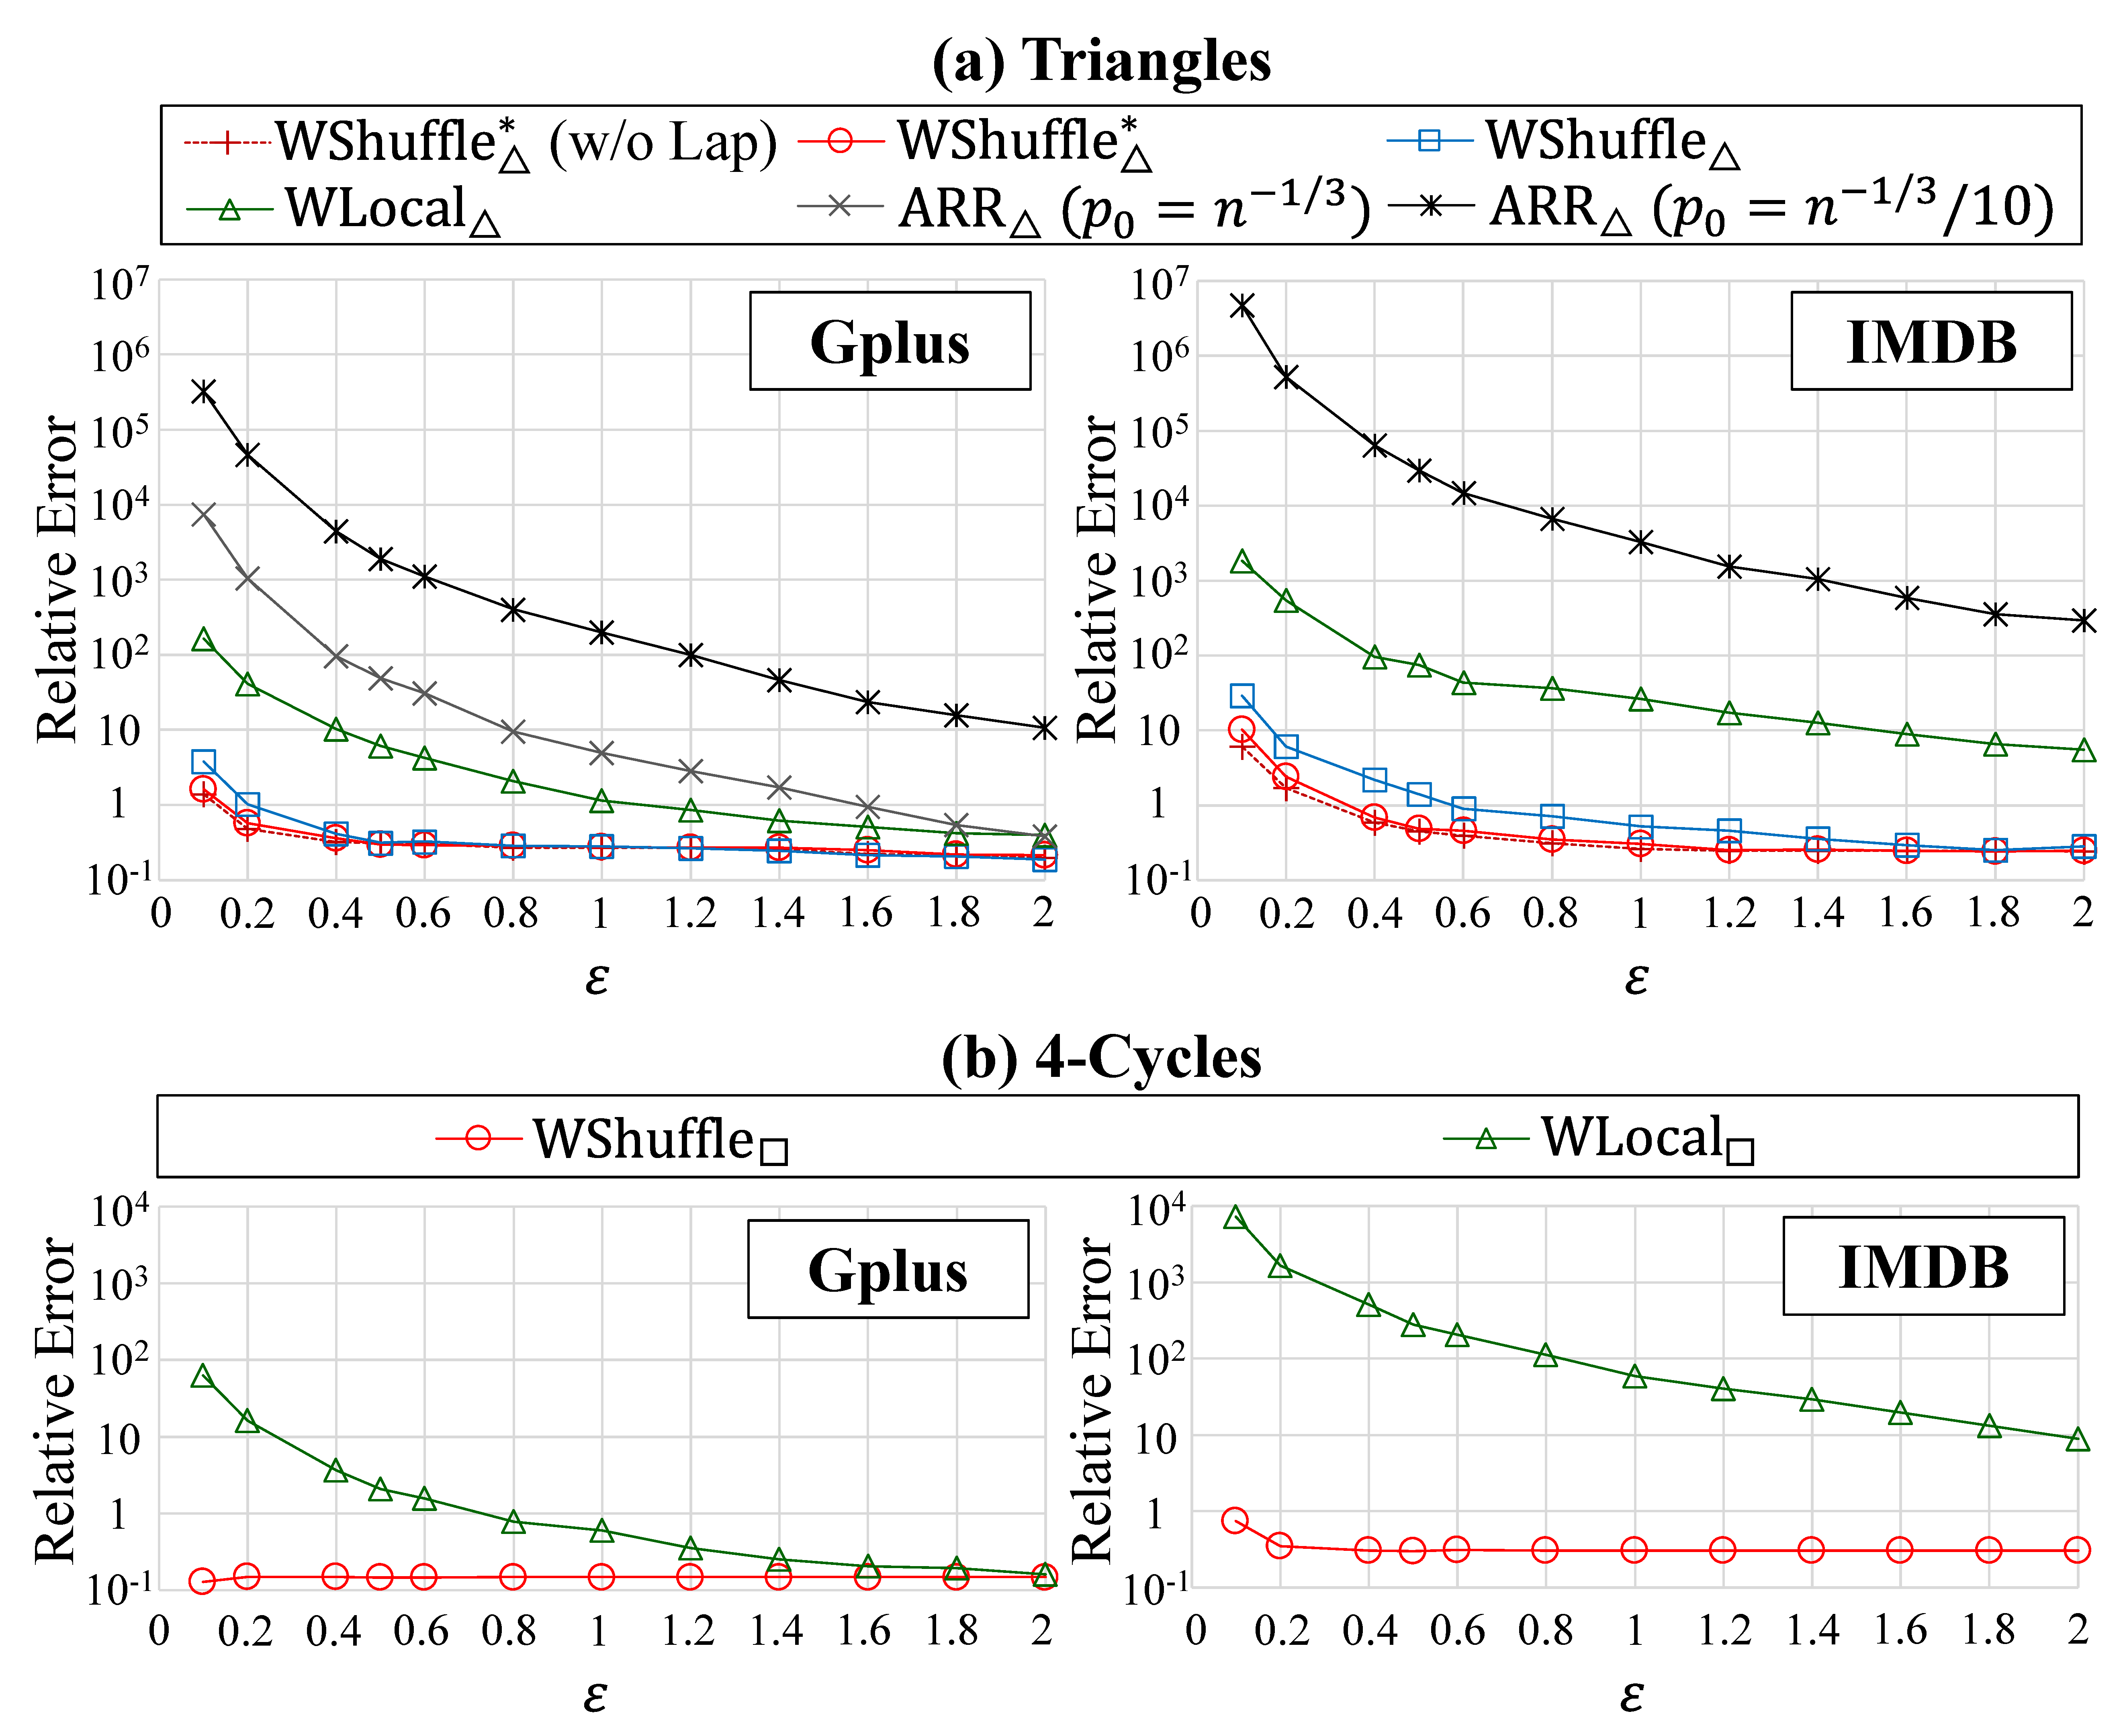
\includegraphics[width=0.99\linewidth]{fig/res1_eps.pdf}
  
  \caption{Relative error vs. $\epsilon$ 
  %in triangle counting 
  ($n=107614$ in \Gplus{}, $n=896308$ in \IMDB{}, $c=1$). 
  $p_0$ is the sampling probability in the ARR. 
  %; numerical bound in \cite{Feldman_FOCS21}). 
  }
  \label{chap3-fig:res1_eps}
\end{figure}

% \begin{table}[t]
%   \centering
%   (a) \Gplus{}\\
%   \begin{tabular}{|c|c|c|c|}
%     \hline
%     & \AlgWSTriVR{} & \AlgWSTri{} & \AlgWSCyc{} \\ \hline
%     $\epsilon=0.5$ & $0.298$ & $0.312$ & $0.145$ \\ \hline
%     $\epsilon=1$ & $0.277$ & $0.279$ & $0.147$ \\ \hline
%   \end{tabular}\\
%   (b) \IMDB{}\\
%   \begin{tabular}{|c|c|c|c|}
%     \hline
%      & \AlgWSTriVR{} & \AlgWSTri{} & \AlgWSCyc{} \\ \hline
%     $\epsilon=0.5$ & $0.488$ & $1.41$ & XX \\ \hline
%     $\epsilon=1$ & $0.308$ & $0.522$ & XX \\ \hline
%   \end{tabular}
%   \caption{Relative error when $\epsilon=0.5$ or $1$ ($n=107614$ in \Gplus{} and $896308$ in \IMDB{}; $c=1$). 
%   }
%   \label{chap3-tab:res1_eps_tri_0.5}
% \end{table}

\begin{table}[t]
  \caption{Relative error (RE) when $\epsilon=0.5$ or $1$ and computational time ($n=107614$ in \Gplus{}, $n=896308$ in \IMDB{}, $c=1$). 
  The lowest relative error is highlighted in bold.
  }
  
  \centering
%   (a) Triangle (\Gplus{})\\
  (a) \Gplus{}\\
  \begin{tabular}{|c|c|c|c|}
    \hline
    & RE ($\epsilon=0.5$) & RE ($\epsilon=1$) & Time (sec)\\ \hline
    \AlgWSTriVR{} & $\bm{2.98 \times 10^{-1}}$ & $\bm{2.77 \times 10^{-1}}$ & $3.60 \times 10^1$ \\ \hline
    \AlgWSTri{} & $3.12 \times 10^{-1}$ & $2.79 \times 10^{-1}$ & $3.62 \times 10^1$ \\ \hline
    \AlgWLTri{} & $6.10 \times 10^0$ & $1.14 \times 10^0$ & $5.83 \times 10^1$ \\ \hline
    \AlgARRTri{} ($p_0=n^{-1/3}$) & $4.90 \times 10^1$ & $4.93 \times 10^0$ & $7.15 \times 10^2$ \\ \hline
    \hspace{-0.5mm}\AlgARRTri{} ($p_0=0.1n^{-1/3}$)\hspace{-0.5mm} & $1.88 \times 10^3$ & $1.97 \times 10^2$ & $3.48 \times 10^1$ \\ \hline \hline
    \AlgWSCyc{} & $\bm{1.45 \times 10^{-1}}$ & $\bm{1.47 \times 10^{-1}}$ & $3.47 \times 10^1$ \\ \hline
    \AlgWLCyc{} & $2.08 \times 10^0$ & $5.96 \times 10^{-1}$ & $5.70 \times 10^1$ \\ \hline
  \end{tabular}\\
%   (b) Triangle (\IMDB{})\\
  (b) \IMDB{}\\
  \begin{tabular}{|c|c|c|c|}
    \hline
    & RE ($\epsilon=0.5$) & RE ($\epsilon=1$) & Time (sec)\\ \hline
    \AlgWSTriVR{} & $\bm{4.88 \times 10^{-1}}$ & $\bm{3.08 \times 10^{-1}}$ & $2.39 \times 10^3$ \\ \hline
    \AlgWSTri{} & $1.41 \times 10^0$ & $5.22 \times 10^{-1}$ & $2.40 \times 10^3$ \\ \hline
    \AlgWLTri{} & $7.46 \times 10^1$ & $2.63 \times 10^1$ & $3.96 \times 10^3$ \\ \hline
    \hspace{-0.5mm}\AlgARRTri{} ($p_0=0.1n^{-1/3}$)\hspace{-0.5mm} & $2.98 \times 10^4$ & $3.27 \times 10^3$ & $2.81 \times 10^3$ \\ \hline \hline
    \AlgWSCyc{} & $\bm{3.03 \times 10^{-1}}$ & $\bm{3.08 \times 10^{-1}}$ & $2.29 \times 10^3$ \\ \hline
    \AlgWLCyc{} & $2.82 \times 10^2$ & $5.91 \times 10^1$ & $3.91 \times 10^3$ \\ \hline
  \end{tabular}
%   (c) 4-cycle (\Gplus{})\\
%   \begin{tabular}{|c|c|c|c|}
%     \hline
%     & RE ($\epsilon=0.5$) & RE ($\epsilon=1$) & Time (sec)\\ \hline
%     \AlgWSCyc{} & $XXX$ & $XXX$ & $XXX$ \\ \hline
%     \AlgWLCyc{} & $XXX$ & $XXX$ & $XXX$ \\ \hline
%   \end{tabular}\\
  \label{chap3-tab:res1_eps_tri_time}
\end{table}

Figure~\ref{chap3-fig:res1_eps} shows the relative error ($c=1$). 
% Here, we used the numerical upper bound in \cite{Feldman_FOCS21} for $\epsilon$ in the shuffle algorithms. 
% We also 
Here, we show the performance of \AlgWSTri{} when we do not add the Laplacian noise (denoted by \AlgWSTri{} (w/o Lap)). 
In \IMDB{}, we do not show \AlgARRTri{} with $p_0 = n^{-1/3}$, because it takes too much time (longer than one day). 
Table~\ref{chap3-tab:res1_eps_tri_time} highlights the relative error when $\epsilon=0.5$ or $1$. 
It also shows the running time of counting triangles or 4-cycles when $\epsilon=1$ (we verified that the running time had little dependence on $\epsilon$). 

Figure~\ref{chap3-fig:res1_eps} and Table~\ref{chap3-tab:res1_eps_tri_time} show that our shuffle algorithms dramatically improve the local algorithms. 
% For example, 
In triangle counting, 
\AlgWSTriVR{} outperforms \AlgWLTri{} by one or two orders of magnitude and \AlgARRTri{} by even more\footnote{Note that \AlgARRTri{} uses only the lower-triangular part of the adjacency matrix $\bmA$ and therefore provides 
% $\epsilon$-edge LDP and 
$\epsilon$-edge DP (rather than $2\epsilon$-edge DP); i.e., it does not suffer from the doubling issue explained in Section~\ref{chap3-sub:privacy}. However, Figure~\ref{chap3-fig:res1_eps} shows that \AlgWSTriVR{} significantly outperforms \AlgARRTri{} 
% with the same privacy budget in edge DP.
even if we double $\epsilon$ for only \AlgWSTriVR{}.}. 
% Although the relative error of \AlgARRTri{} can be improved by using a larger $p_0$, it results in longer running time. 
\AlgWSTriVR{} also requires less running time than \AlgARRTri{} with $p_0 = n^{-1/3}$. 
Although the running time of \AlgARRTri{} can be improved by using a smaller $p_0$, it results in a higher relative error. 
% Similarly, 
In 4-cycle counting, 
\AlgWSCyc{} significantly outperforms \AlgWLCyc{}. 
The difference between our shuffle algorithms and the local algorithms is larger in \IMDB{} because it is more sparse; i.e., the difference between $d_{max}$ and $n$ is larger in \IMDB{}. 
This is consistent with our theoretical results in Tables~\ref{chap3-tab:upper_bounds_triangle} and \ref{chap3-tab:upper_bounds_4cycle}. 

Figure~\ref{chap3-fig:res1_eps} and Table~\ref{chap3-tab:res1_eps_tri_time} also show that \AlgWSTriVR{} outperforms \AlgWSTri{}, especially when $\epsilon$ is small. 
% or the dataset is sparse, i.e., \IMDB{}. 
This is because the variance is large when $\epsilon$ is small. 
In addition, \AlgWSTriVR{} significantly outperforms \AlgWSTri{} in \IMDB{} because \AlgWSTriVR{} significantly reduces the variance when $d_{max} \ll n$, as shown in Table~\ref{chap3-tab:upper_bounds_triangle}. 
In other words, this is also consistent with our theoretical results. 
For example, when $\epsilon=0.5$, our variance reduction technique reduces the relative error from $1.41$ to $0.488$ (about one-third) in \IMDB{}. 

Furthermore, Figure~\ref{chap3-fig:res1_eps} shows that the relative error of \AlgWSTriVR{} is hardly changed by adding the Laplacian noise. 
This is because the sensitivity of each user's degree $d_i$ is very small ($=1$). 
In this case, the Laplacian noise is also very small. 

\begin{figure}[t]
  \centering
  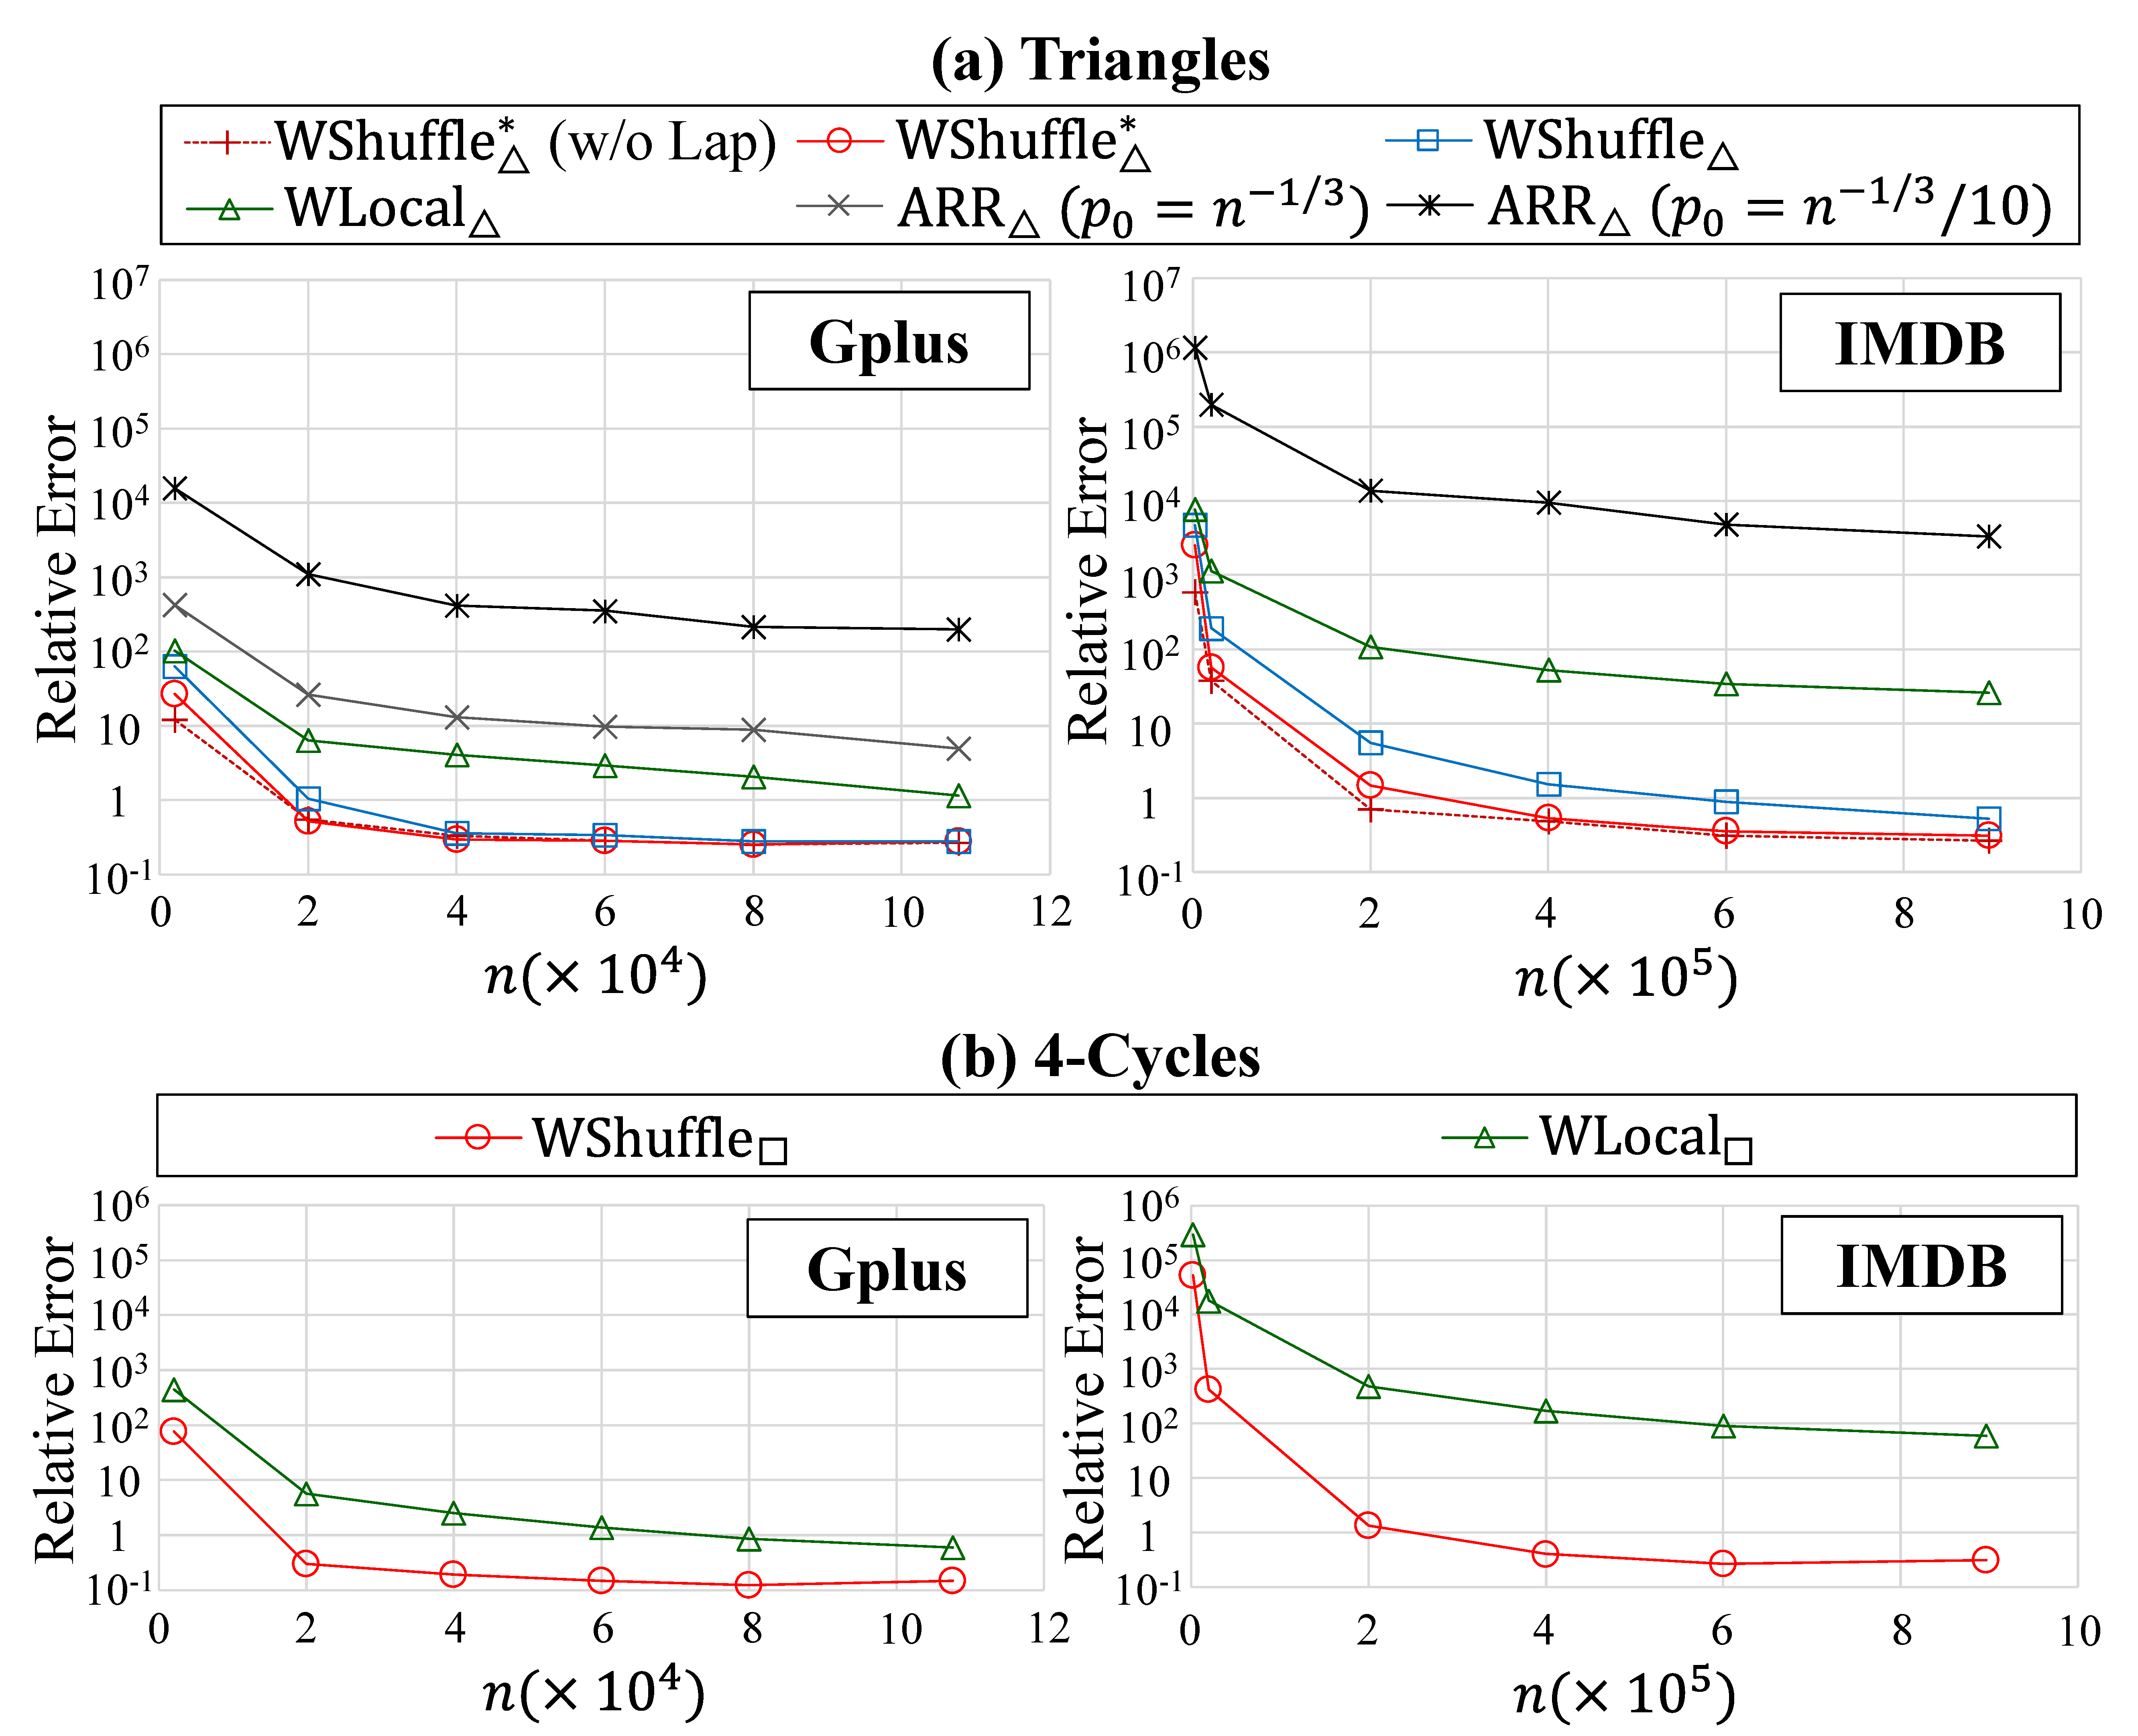
\includegraphics[width=0.99\linewidth]{fig/res2_n.pdf}
  
  \caption{Relative error vs. $n$ ($\epsilon=1$, $c=1$).
  }
  \label{chap3-fig:res2_n}
\end{figure}

% Table~\ref{chap3-tab:res1_eps_tri_time} shows that 
Our \AlgWSTriVR{} achieves a relative error of $0.3$ ($\ll 1$) 
% and \AlgWSCyc{} achieve relative errors of $0.15$ to $0.3$ ($\ll 1$) 
% with a reasonable privacy budget -- $\epsilon = 0.5$ or $1$ in element DP and $2\epsilon = 1$ or $2$ in edge DP. 
when the privacy budget is $\epsilon = 0.5$ or $1$ in element DP ($2\epsilon = 1$ or $2$ in edge DP). 
\AlgWSCyc{} achieve a relative error of $0.15$ to $0.3$ with a smaller privacy budget (e.g., $\epsilon = 0.2$) because it  does not send local edges -- the error of \AlgWSCyc{} is mainly caused by user-pair sampling that is independent of $\epsilon$. 

In summary, our \AlgWSTriVR{} and \AlgWSCyc{} significantly outperform the local algorithms and achieve a relative error much smaller than $1$ with a reasonable privacy budget, i.e., $\epsilon \leq 1$. 

\smallskip
\noindent{\textbf{Relative Error vs. $n$.}}~~Next, we evaluated the relation between the relative error and $n$. 
% the number $n$ of users. 
Specifically, we randomly selected $n$ users from all users and extracted a graph with $n$ users. 
Then we set $\epsilon = 1$ and changed $n$ to various values starting from $2000$. 
%from $2000$ to $107614$ and $896308$ in \Gplus{} and \IMDB{}, respectively. 

Figure~\ref{chap3-fig:res2_n} shows the results ($c=1$). 
% We observe that 
When $n=2000$, \AlgWSTri{} and \AlgWSCyc{} provide 
%almost the same relative error as 
relative errors close to \AlgWLTri{} and \AlgWLCyc{}, respectively. 
This is because the privacy amplification effect is limited when $n$ is small. 
For example, when $n=2000$ and $\epsilon=1$, 
% and $\delta=10^{-8}$, 
the numerical bound is $\epsilon_L=1.88$. 
The value of $\epsilon_L$ increases with increase in $n$; e.g., when $n=107614$ and $896308$, the numerical bound is $\epsilon_L= 5.86$ and $7.98$, respectively. 
This explains the reason that our shuffle algorithms significantly outperform the local algorithms when $n$ is large in Figure~\ref{chap3-fig:res2_n}. 
% the large difference between our shuffle algorithms and the local algorithms. 
% in Figure~XX. 

% Figure~XX also shows that the relative error decreases with increase in $n$. 
% There are two reasons for this: (i) the squares of the true triangle and 4-cycle counts are $O(n^2 d_{max}^4)$ and $O(n^2 d_{max}^6)$, respectively; (ii) $d_{max}$ is proportional to $n$, as we randomly selected $n$ users from all users. 


% \smallskip
% \noindent{\textbf{Clustering Coefficient.}}~~TBD

\smallskip
\noindent{\textbf{Parameter $c$ in \AlgWSTriVR{}.}}~~Finally, we evaluated our \AlgWSTriVR{} while changing the parameter $c$ that controls the bias and variance. 
% of the estimate. 
Recall that as $c$ increases, the bias is increased, and the variance is reduced. 
We set $\epsilon=0.1$ or $1$ and changed $c$ from $0.1$ to $4$. 

Figure~\ref{chap3-fig:res4_thr} shows the results. 
Here, we also show the relative error of \AlgWSTri{}. 
We observe that the optimal $c$ is different for $\epsilon=0.1$ and $\epsilon=1$. The optimal $c$ is around $3$ to $4$ for $\epsilon=0.1$, whereas the optimal $c$ is around $0.5$ to $1$ for $\epsilon=1$. 
This is because the variance of \AlgWSTri{} is large (resp.~small) when $\epsilon$ is small (resp.~large). 
For a small $\epsilon$, a large $c$ is effective in significantly reducing the variance. 
For a large $\epsilon$, a small $c$ is effective in keeping a small bias. 
% The optimization of $c$ in \AlgWSTriVR{} is an interesting future research direction. 

We also observe that \AlgWSTriVR{} is always better than (or almost the same as) \AlgWSTri{} when $c=1$ or $2$. 
This is because most users' degrees are smaller than the average degree $d_{avg}$, as described in Section~\ref{chap3-sub:var_red}. 
When $c=1$ or $2$, most user-pairs are ignored. 
Therefore, we can significantly reduce the variance at the cost of a small bias. 

\begin{figure}[t]
  \centering
  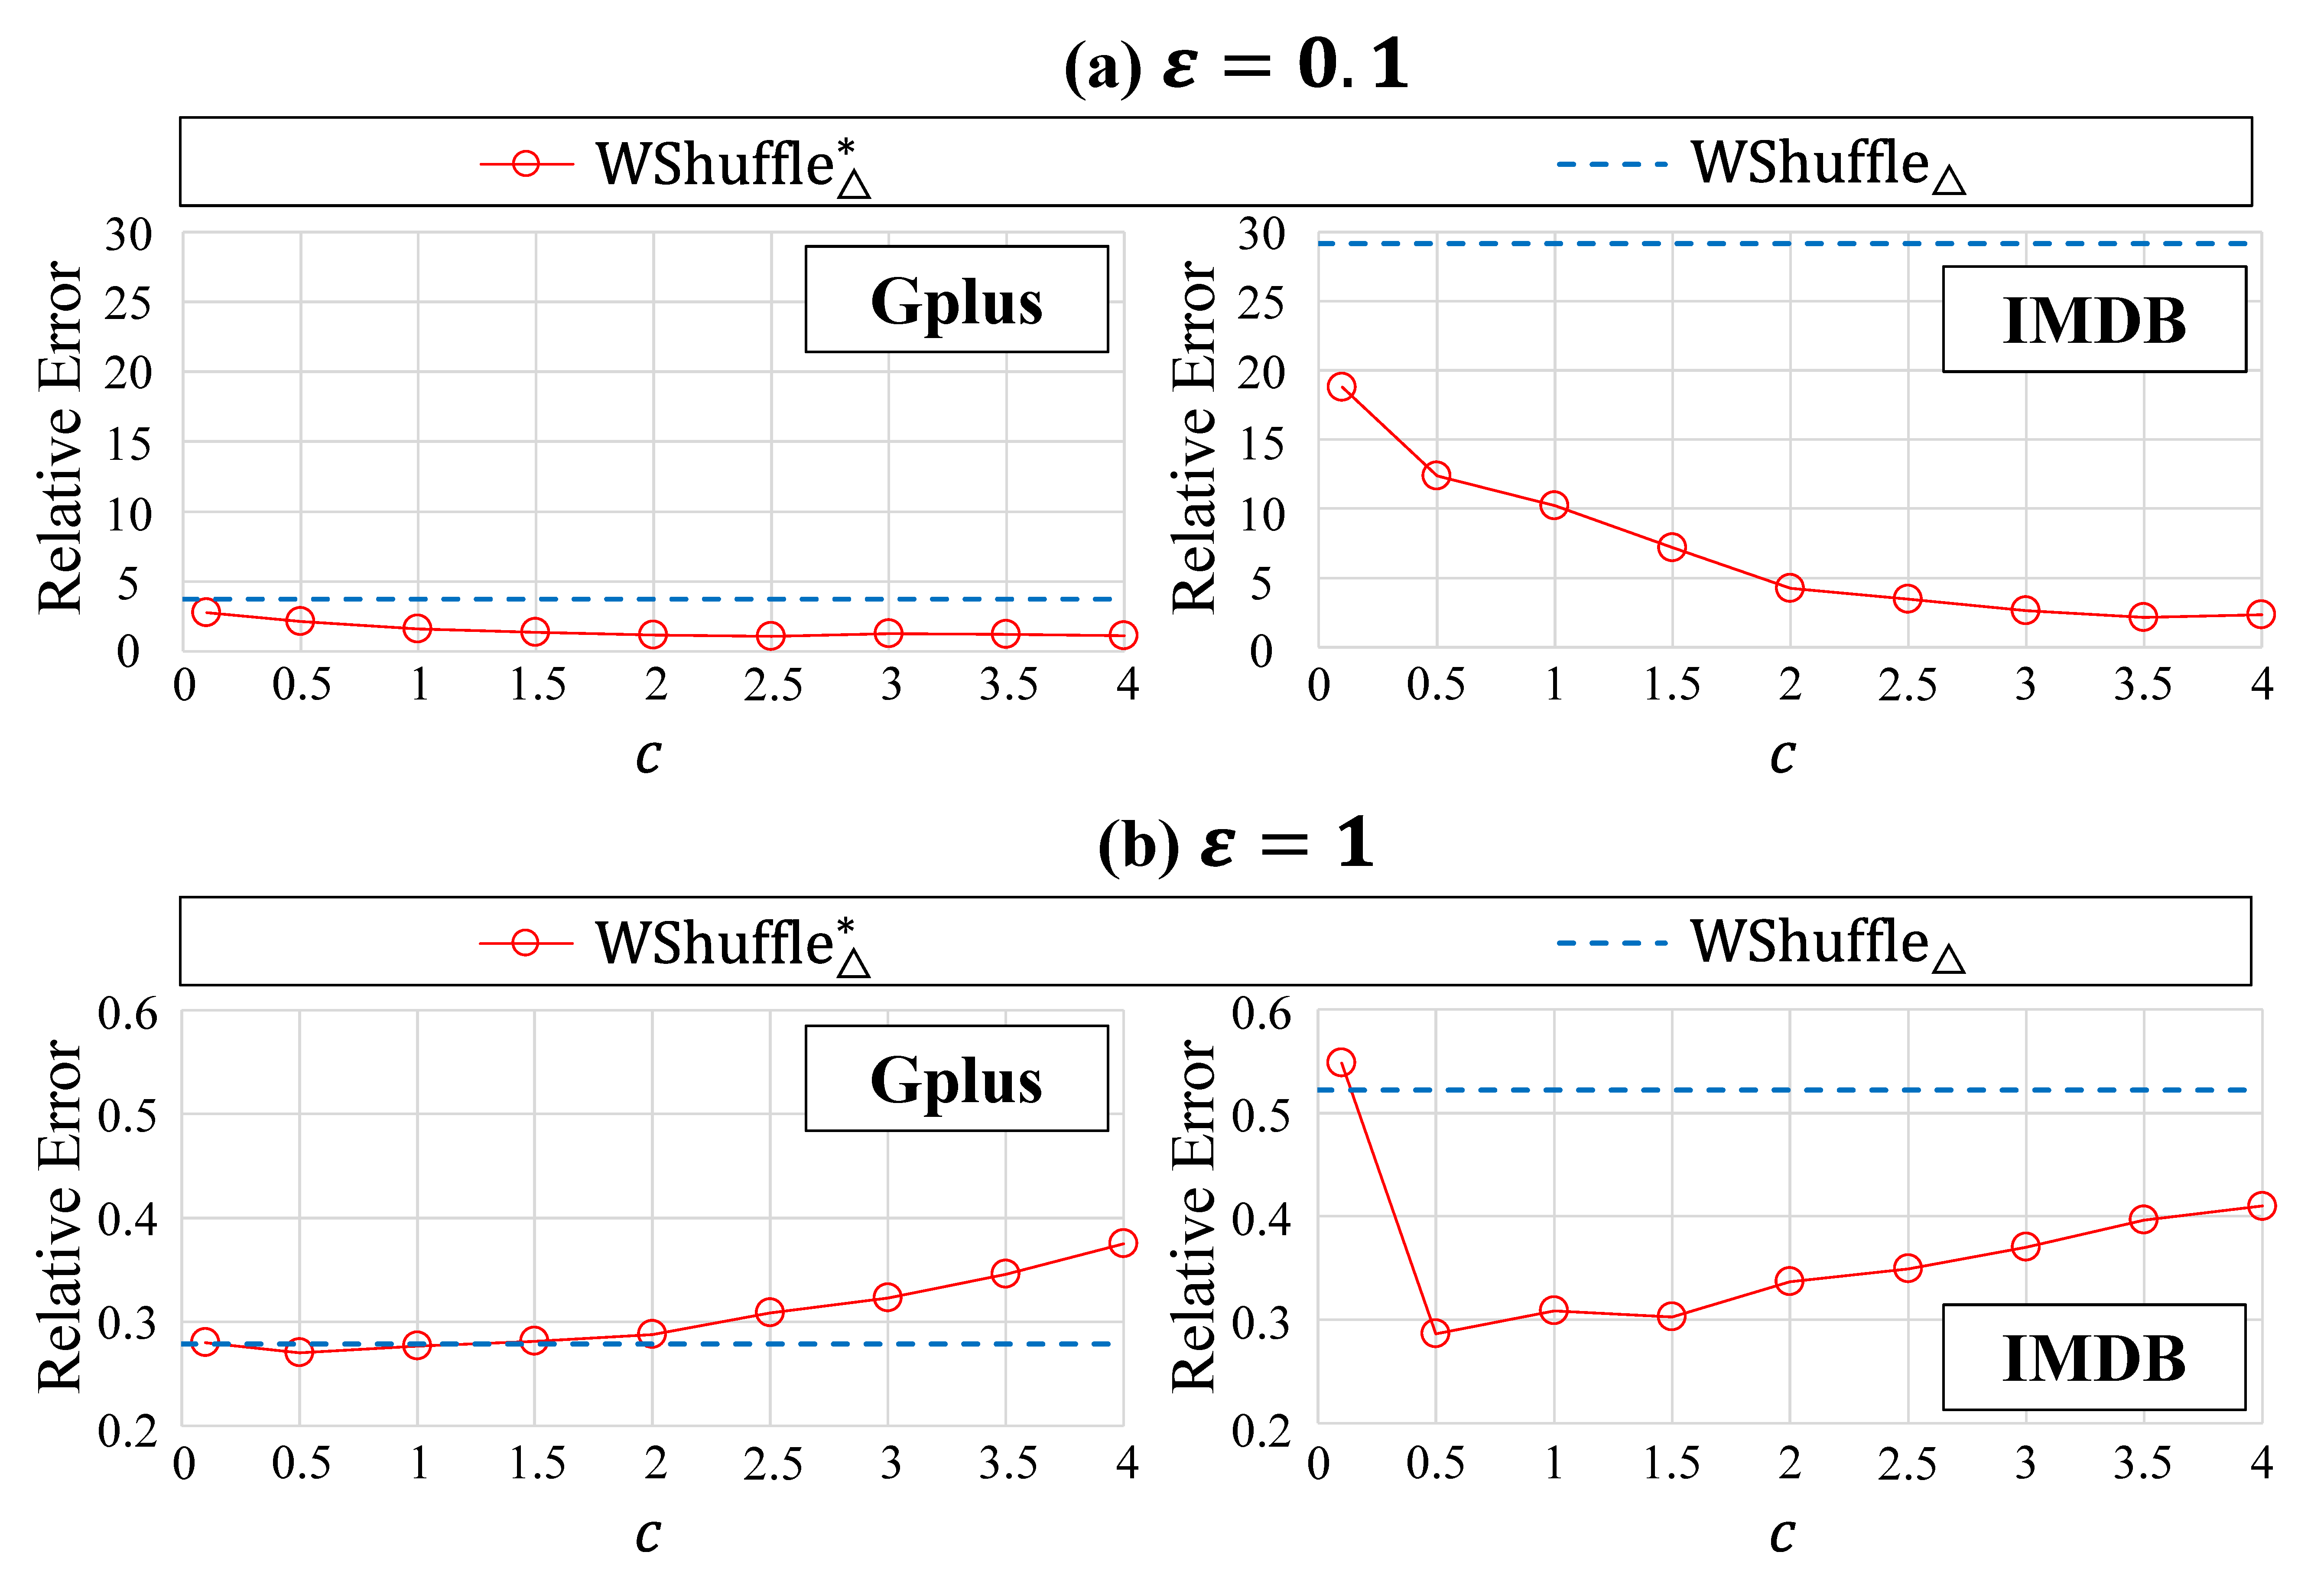
\includegraphics[width=0.99\linewidth]{fig/res4_thr.pdf}
  
  \caption{Relative error vs. parameter $c$ in \AlgWSTriVR{} ($n=107614$ in \Gplus{}, $n=896308$ in \IMDB{}).
  }
  \label{chap3-fig:res4_thr}
\end{figure}

\smallskip
\noindent{\textbf{Summary.}}~~In summary, our answers to the three questions at the beginning of Section~\ref{chap3-sec:experiments} are as follows. 
RQ1: Our \AlgWSTriVR{} and \AlgWSCyc{} outperform the one-round local algorithms by one or two orders of magnitude (or even more). 
% \AlgWSTriVR{} is even comparable to the two-rounds local algorithm in \cite{Imola_USENIX22} (\AlgTwoRS{}) that requires a lot of user effort 
% and synchronization 
% in terms of accuracy. 
RQ2: Our variance reduction technique significantly reduces the relative error (e.g., by about one-third) 
for a small $\epsilon$ in a sparse dataset. 
% when $\epsilon$ is small or the dataset is sparse. 
RQ3: 
% Our \AlgWSTriVR{} and \AlgWSCyc{} achieve a relative error of $0.15$ to $0.3$ ($\ll 1$) when $\epsilon=0.5$ or $1$ in element DP ($2\epsilon=1$ or $2$ in edge DP). 
\AlgWSTriVR{} achieves a relative error of $0.3$ ($\ll 1$) when $\epsilon=0.5$ or $1$ in element DP ($2\epsilon=1$ or $2$ in edge DP). 
\AlgWSCyc{} achieves a relative error of $0.15$ to $0.3$ with a smaller privacy budget: $\epsilon=0.2$. 